\chapter{Modeling true concurrency geometrically}
\label{chap:geomod}



We have seen in the previous chapter several abstract formalisms to talk about true concurrency, that is, concurrent systems in which processes can do actions simultaneously. In particular, we have seen higher dimensional automata, which are on top of the hierarchy of expressiveness. HDA are, by nature, very geometric. The underlying precubical set can be thought as a collection of cubes of any dimensions which represent the truly concurrent behaviors of the system: an n-cube models n actions that can be done simultaneously. In this chapter, we formalize this geometric idea. We associate a precubical set with different geometric objects, defined by glueing together (real) cubes. We start, in Section \ref{sec:georea}, by doing it in topological spaces. This allows us to relate intuitions from HDA and from topology. The only problem is directedness: transitions of HDA are directed while topological spaces are not. So the Section \ref{sec:sevdir} is dedicated to looking at different ways to add directedness. We will mainly see two ways and compare them: firstly with the idea of defining an order locally and assuring global consistency, this leads to streams \cite{krishnan09} ; and then by specifying particular paths that we consider directed, this leads to d-spaces \cite{grandis09}. We will then see, in Section \ref{sec:geovi}, how to geometrically study concurrent programs, defining directed homotopies and fundamental categories. Finally, in Section \ref{sec:traspa}, we look at another important construction which somehow formalizes a ``space of executions'' in directed spaces, the trace space from \cite{fahrenberg07}.


\section{Geometric realizations}
\label{sec:georea}

The general idea is to \textbf{realize} precubical sets in topological spaces. In the following, we denote by $\topo$ the category of topological spaces and continuous functions. The \textbf{standard topological cube of dimension $n$}, denoted $\Box_n$, is the product space $[0,1]^n$. A \textbf{face map} is a continuous function of the form $\map{d_i^\alpha}{\Box_{n-1}}{\Box_n}$ with $1 \leq i \leq n$ and $\alpha \in \{0,1\}$ such that $$d_i^\alpha(t_1, \ldots, t_{n-1}) = (t_1, \ldots, t_{i-1}, \alpha, t_i, \ldots, t_{n-1}).$$

The \textbf{geometric realization} of a precubical set $(X,\partial)$, denoted $\geo{X}$, is the disjoint union $\bigsqcup\limits_{n\in\nat} X_n\times\Box_n$ quotiented by the smallest equivalence relation $\sim$ such that for every $n \in \nat^\star$, every $ 1 \leq i \leq n$, every $\alpha \in \{0,1\}$, every $x \in X_n$ and every $\mathbf{t} \in \Box_{n-1}$, 
$$(\partial_i^\alpha(x), \mathbf{t}) \sim (x, d_i^\alpha(\mathbf{t})).$$

For example, the geometric pictures of HDA in the previous chapter are geometric realizations. Actually, those examples were really non-degenerated. More complicated phenomena can occur: for example, a cube may have different faces which are identified. For example, with $X_2 = \{c\}$, $X_1 = \{s_1,s_2,s_3\}$, $X_0 = \{p_1,p_2\}$, we can construct a hollow cylinder:
	\begin{figure}[H]
		\begin{center}
    			\begin{tikzpicture}[auto,scale = 1]
		\draw (0,0) rectangle (3,3);
		\node at (1.5,1.5) {$c$};
		\node at (1.5,-0.3) {$s_1$};
		\node at (1.5,3.3) {$s_2$};
		\node at (-0.3,1.5) {$s_3$};
		\node at (3.3,1.5) {$s_3$};
		\node at (-0.3,-0.3) {$p_1$};
		\node at (3.3,-0.3) {$p_1$};
		\node at (-0.3,3.3) {$p_2$};
		\node at (3.3,3.3) {$p_2$};
		
		\draw (7,3) ellipse (1.25 and 0.5);
		\draw (5.75,0) -- (5.75,3);
		\draw (5.75,0) arc (180:360:1.25 and 0.5);
		\draw [dashed] (5.75,0) arc (180:360:1.25 and -0.5);
		\draw (8.25,3) -- (8.25,0); 
		\node at (7,1.5) {$c$};
		\node at (8.55,1.5) {$s_3$};
		\node at (7,-0.8) {$s_1$};
		\node at (7,3.8) {$s_2$};
\end{tikzpicture}
  		\end{center}
  		%\caption{}
  		%\label{}
	\end{figure}
\noindent  with $\partial_1^0(c) = s_1$, $\partial_1^1(c) = s_2$, $\partial_2^0(c) = \partial_2^1(c) = s_3$, and one can construct more twisted spaces like the M�bius strip:
	\begin{figure}[H]
		\begin{center}
    			\begin{tikzpicture}[auto,scale = 1]
		\draw (0,0) rectangle (3,3);
		\draw (3,0) rectangle (6,3);
		\node at (1.5,1.5) {$c_1$};
		\node at (4.5,1.5) {$c_2$};
		\node at (1.5,-0.3) {$s_1$};
		\node at (4.5,-0.3) {$s_3$};
		\node at (1.5,3.3) {$s_2$};
		\node at (4.5,3.3) {$s_4$};
		\node at (-0.3,1.5) {$s_5$};
		\node at (6.3,1.5) {$s_5$};
		\node at (3.3,1.5) {$s_6$};
		\node at (-0.3,-0.3) {$p_1$};
		\node at (-0.3,3.3) {$p_2$};
		\node at (6.3,3.3) {$p_1$};
		\node at (3,-0.3) {$p_3$};
		\node at (6.3,-0.3) {$p_2$};
		\node at (3,3.3) {$p_4$};
		\node at (-1.5,-1.5) {};
\end{tikzpicture}
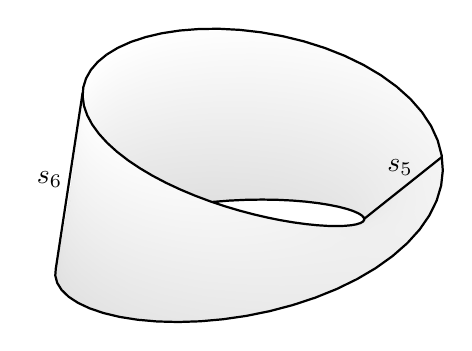
\begin{tikzpicture}

\begin{axis}[
    hide axis,
    view={40}{40}
]
\addplot3 [
    surf, shader= interp,%shader=faceted interp,
    %point meta=x,
    colormap = {whiteblack}{color(0cm)  = (gray!25);color(1cm) = (white)},
    %colormap/whiteblack,
    samples=30,
    samples y=5,
    z buffer=sort,
    domain=0:360,
    y domain=-0.5:0.5
] (
    {(1+0.5*y*cos(x/2)))*cos(x)},
    {(1+0.5*y*cos(x/2)))*sin(x)},
    {0.5*y*sin(x/2)});

\addplot3 [
    samples=50,
    domain=-140:180, % The domain needs to be adjusted manually, depending on the camera angle, unfortunately
    samples y=0,
    thick
] (
    {(1+0.5*0.5*cos(x/2)))*cos(x)},
    {(1+0.5*0.5*cos(x/2)))*sin(x)},
    {0.5*0.5*sin(x/2)});
    
    \addplot3 [
    samples=50,
    domain=-180:138, % The domain needs to be adjusted manually, depending on the camera angle, unfortunately
    samples y=0,
    thick
] (
    {(1+0.5*-0.5*cos(x/2)))*cos(x)},
    {(1+0.5*-0.5*cos(x/2)))*sin(x)},
    {0.5*-0.5*sin(x/2)});
\end{axis}

\draw[thick] (0.93,1.92) -- (1.27,4.15);
\node at (0.85,3.05) {$s_6$};
\draw[thick] (4.85,2.55) -- (5.83,3.33);
\node at (5.3,3.2) {$s_5$};

\end{tikzpicture}





  		\end{center}
  		%\caption{}
  		%\label{}
	\end{figure}
\vspace{-1cm}
 \noindent or even a projective plane: the geometry of such a realization may be very intricate.
 
 
 There is a more abstract and general way to define geometric realization which will be useful later. Denote by $\Box$ the category whose: 
 \begin{itemize}
 	\item objects are natural numbers,
	\item morphisms from $n$ to $m$ are pairs $(f,t)$ where:
 		\begin{itemize}
			\item $\map{f}{\{0,\ldots, n\}}{\{0,\ldots,m\}}$ is an injective and monotone function,
			\item $\map{t}{\{0,\ldots, m\}\setminus \text{Im}(f)}{\{0,1\}}$,
		\end{itemize}
	\item composition $(g,s)\circ (f,t)$ is $(g\circ f, s \shuffle t)$ with $\map{(f,t)}{n}{m}$ and $\map{(g,s)}{m}{p}$, where $\map{s \shuffle t}{\{0,\ldots, p\}\setminus \text{Im}(g\circ f)}{\{0,1\}}$ maps $i \notin \text{Im}(g)$ to $s(i)$ and $i \in \text{Im}(g)\setminus\text{Im}(g\circ f)$ to $t(j)$ with $g(j) = i$.
\end{itemize}
A precubical set is then a functor from $\Box^{op}$ to $\setcat$, i.e., a presheaf on $\Box$. Since the category of presheaves $\psh{\Box}$ is the free cocompletion of $\Box$, given a functor $\map{F}{\Box}{\C}$ where $\C$ is cocomplete, leads to a unique functor $\map{\widehat{F}}{\psh{\Box}}{\C}$ such that $\widehat{F}\circ y_\Box = F$, where $y_\Box$ is the Yoneda embedding. $\text{Geom}$ can be obtained as $\widehat{G}$ where $\map{G}{\Box}{\topo}$ maps $n$ to $\Box_n$ and $\map{(f,t)}{n}{m}$ to the continuous function from $\Box_n$ to $\Box_m$ which maps $(u_1,\ldots,u_n)$ to $(v_1, \ldots, v_m)$ where $v_i = u_{f(j)}$ if $i \in \text{Im}(f)$, $v_i = t(i)$ otherwise.
		
 
 The interest of this realization is to think of concurrent systems geometrically:
 \begin{itemize}
 	\item a state is just a point,
	\item an execution is a path, i.e. a continuous function from the segment $[0,1]$ to $\geo{X}$,
	\item homotopy seen for HDA can be defined continuously: given two paths $\gamma, \rho$ such that $\gamma(0) = \rho(0) = a$ and $\gamma(1) = \rho(1) = b$ (we say that $\gamma, \rho$ go from $a$ to $b$ and note $\pathto{\gamma,\rho}{a}{b}$), a homotopy $H$ between $\gamma$ and $\rho$ is a continuous function $$\map{H}{[0,1]\times[0,1]}{\geo{X}}$$ such that:
		\begin{itemize}
			\item $H(t,0) = a$ and $H(t,1) = b$ for all $t \in [0,1]$,
			\item $H(0,t) = \gamma(t)$ and $H(1,t) = \rho(t)$ for all $t \in [0,1]$.
		\end{itemize}
\end{itemize}

More generally, given a topological space $X$, a \textbf{path in $X$} is a continuous function from $[0,1]$ to $X$. We note $\pathsp{X}$ the set of paths in $X$. It can be equipped with a topology, the compact-open topology, whose open sets are generated by the $$[K,U] = \{\gamma \mid \gamma(K) \subseteq U\}$$
with $K$ compact of $[0,1]$ and $U$, an open set of $X$. For $a, b \in X$, we denote by $\pathspp{X}{a}{b}$ the subspace of paths from $a$ to $b$. A \textbf{homotopy} between $\gamma$ and $\rho \in \pathspp{X}{a}{b}$ is then a path in $\pathspp{X}{a}{b}$ from $\gamma$ to $\rho$. In this case, we say that $\gamma$ and $\rho$ are homotopic, and we note $[\gamma]$ the equivalence class of $\gamma$.


There is still a flaw in this geometric view of concurrency: non-directedness. The problem is that transitions, for example in a HDA, are directed: there is a source and a target. Those transitions are geometrically modeled as a segment $[0,1]$ with the source mapped on $0$ and the target on $1$. This segment is not directed in the sense that one can define a path from $1$ to $0$, meaning that one can follow transitions backwardly, which is not possible in a HDA. So paths are not the good way to model executions but directed paths are. The goal of the following chapter (and of directed algebraic topology in general) will be to add this directedness into the definition of topological spaces to define nice notions of directed spaces. 


\section{Several ways of modeling directedness}
\label{sec:sevdir}

The general idea will be to add some extra structures to the topological spaces being used. We will see different ways to do so in the following. We will define cocomplete categories of ``directed spaces'' $\D$, which have a natural ``forgetful functor'' $\mathcal{U}$ to topological spaces. A crucial property of this forgetful functor would be that it preserves colimits. Indeed, in this case, if one can provide a functor $\map{G'}{\Box}{\D}$, such that $\mathcal{U}\circ G' = G$ as defined in the previous subsection, then the unique functor $\widehat{G'}$ will satisfy that $\mathcal{U}\circ\widehat{G'} = \text{Geom}$ and will be a candidate of a realization of precubical sets in directed spaces. A way to assure that it preserves colimits is to assure that it has a right adjoint, or even better, that it is a topological functor \cite{adamek04}. The idea of a topological functor $F$ is that every antecedent of an object corresponds to a way of adding some structure on this object. Moreover, those ways should naturally be ordered by the quantity of structures added in such a way that we can talk about the ``coarsest structure such that ...''. A typical example is the forgetful functor from topological spaces to sets. A topological functor always has a right adjoint (given by the finest structure) and a left adjoint (given by the coarsest structure). More precisely, given a functor $\map{F}{\C}{\D}$, the \textbf{fiber over $d$}, is the class of objects of $\C$ such that $F(c) = d$. This fiber over $d$ is ordered by $c \leq c'$ if and only if there is a morphism from $\map{f}{c}{c'}$ with $F(f) = \text{id}_d$. We say that $F$ is \textbf{topological} if:
\begin{itemize}
	\item it is faithful,
	\item for every fiber over an object of $\D$, $\leq$ is a partial order,
	\item for every object $d$ of $\D$, and every collection of morphisms $(\map{g_i}{d}{F(c_i)})_{i \in I}$ there is an object $c$ of $\C$ such that $F(c) = d$ and a collection of morphisms $(\map{f_i}{c}{c_i})_{i\in I}$ with $F(f_i) = g_i$ such that for every morphism $\map{h}{F(c')}{F(c)}$, if for every $i \in I$, there is a morphism $\map{h_i}{c'}{c_i}$ with $F(h_i) = g_i\circ h$, then there is $\map{h'}{c'}{c}$ with $F(h') = h$.
\end{itemize}

For example, the forgetful functor $\map{\mathcal{U}}{\topo}{\setcat}$ is topological. Given a set $X$ and two topologies $O_1$ and $O_2$ on $X$, $X,O_1 \leq X,O_2$ if and only if the identity function is continuous, considering $O_1$ as the topology on the domain, and $O_2$ on the image. This means that elements of $O_2$ (which are open sets for this topology) are also elements of $O_1$. This means that $X,O_1 \leq X,O_2$ if and only if $O_2 \subseteq O_1$ and so $\leq$ is a partial order. Given a collection of functions $(\map{g_i}{X}{Y_i})_{i \in I}$ where $Y_i$ are topological space, there is a coarsest topology on $X$ that makes the $g_i$ continuous: this is the topology generated by the $g_i^{-1}(U)$ with $U$ open set of $Y_i$. This coarsest topology is the object $c$ required in the third point of the definition of a topological functor.

	\subsection{PO-spaces}
	
	Let us start with a simple idea:
	
	\begin{defi}
	A \textbf{partially ordered space} (po-space for short) is a topological space $X$ with a partial order $\leq$ on it. A \textbf{dimap} between po-spaces is a continuous monotone function between them. We note $\potop$ the category of po-spaces and dimaps.
	\end{defi}
	
	Usually, one says `po-space' for a topological space with a closed partial order on it \cite{nachbin65}, but as this closure property is not useful in our study, we will omit it from our definition. 
	
	$\Box_n$ can be equipped with a partial order, namely the product (or component-wise) order. The face maps $d_i^\alpha$ are then dimaps, and so this defines a functor $\map{G'}{\Box}{\potop}$. By a \textbf{directed path in $X$} (or \textbf{dipath} for short) we mean a dimap from $[0,1]$, with its usual ordering, to $X$. The dipaths of $\Box_n$ are then component-wise increasing paths.
	
	There is a forgetful functor from $\potop$ to $\topo$ which forgets the partial order. It satisfies the first two conditions of a topological functor, since the ordering $\leq$ denotes the inverse inclusion of the partial orders. $\potop$ is cocomplete and the colimits are computed as follow: let $\map{D}{\D}{\potop}$ be a small diagram. Forgetting the partial order, this diagram has a colimit in $\topo$, let us note it $X$, which is the space
	$$\bigsqcup\limits_{d \in \ob{\D}} D(d) / \sim$$
where $\sim$ is the smallest equivalence relation such that for every $\map{f}{d}{d'}$ morphism of $\D$, for every $x \in D(d)$, $x \sim D(f)(x)$, equipped with the quotient topology. We note $\map{p_d}{D(d)}{X}$ the quotient maps. $X$ can be equipped with a preorder $\sqsubseteq$, with $\alpha \sqsubseteq \beta$ if and only if there is a sequence $\alpha = \gamma_1$, \ldots, $\gamma_n = \beta$ such that for every $i \in \{1, \ldots, n-1\}$, there $x_i$ and $y_i$ in some $D(d_i)$ with $x_i \leq y_i$ in $D(d_i)$, $p_{d_i}(x_i) = \gamma_i$ and $p_{d_i}(y_i) = \gamma_{i+1}$. The preorder $\sqsubseteq$ may not be a partial order. For example, with this diagram:\\
	\begin{figure}[H]
		\begin{center}
    			
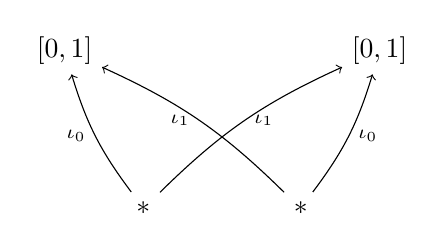
\begin{tikzpicture}[scale=1]
		
	\node (1) at (0,0) {$\ast$};
	\node (2) at (2,0) {$\ast$};
	\node (3) at (-1,2) {$[0,1]$};
	\node (4) at (3,2) {$[0,1]$};
	
	\path[->,font=\scriptsize, bend left = 10]
		(1) edge node[left]{$\iota_0$} (3)
		(1) edge node[right]{$\iota_1$} (4);
		
	\path[->,font=\scriptsize, bend right = 10]
		(2) edge node[left]{$\iota_1$} (3)
		(2) edge node[right]{$\iota_0$} (4);
			
\end{tikzpicture}


  		\end{center}
  		%\caption{}
  		%\label{}
	\end{figure}
\noindent where $\ast$ is a point space and $\iota_\alpha$ is the function that maps $\ast$ to $\alpha$, $X$ is homeomorphic to a circle:\\
	\begin{figure}[H]
		\begin{center}
    			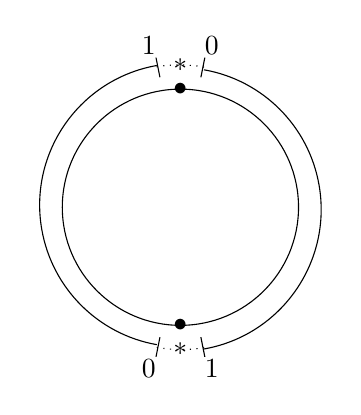
\begin{tikzpicture}[auto,scale = 1]

		\draw (0,0) circle (1.5cm);
		\node at (0,1.5) {$\bullet$};
		\node at (0,-1.5) {$\bullet$};
		\node at (0,1.8) {$\ast$};
		\node at (0,-1.8) {$\ast$};
		\draw (0.3,-1.8) arc (-80:80:1.8cm);
		\draw (-0.3,1.8) arc (100:260:1.8cm);
		\draw (0.26,1.65) -- (0.31,1.9);
		\draw (-0.26,1.65) -- (-0.31,1.9);
		\draw (0.26,-1.65) -- (0.31,-1.9);
		\draw (-0.26,-1.65) -- (-0.31,-1.9);
		\node at (0.40,2.05) {$0$};
		\node at (0.40,-2.05) {$1$};
		\node at (-0.40,2.05) {$1$};
		\node at (-0.40,-2.05) {$0$};
		\draw[dotted] (0.3,1.78) arc (80:100:1.8cm);
		\draw[dotted] (-0.3,-1.78) arc (260:280:1.8cm);
		
\end{tikzpicture}
  		\end{center}
  		%\caption{}
  		%\label{}
	\end{figure}
\noindent and $\sqsubseteq \, = X\times X$.

Denote by $\equiv$ the relation such that $\alpha \equiv \beta$ if and only if $\alpha \sqsubseteq \beta$ and $\beta \sqsubseteq \alpha$, and $Y = X/\equiv$, equipped with the quotient topology and the quotient order (which is a partial order this time). Then $Y$ is the colimit of $D$ in $\potop$. 

Remark that, from this computation, the forgetful functor does not preserve colimits. Indeed, considering the previous example, its colimit in $\topo$ is a circle, while its colimit in $\potop$ is a point. We could have avoided this problem by considering preorder instead of partial order. The problem is still here: we would expect that the glueing of two directed segments as in this example would give us somehow a ``directed circle'', i.e., a circle on which one can only turn in one direction, but the colimit is a circle on which every path is directed.
	
	\subsection{Local PO-spaces}
	
	We have seen that the main problem of po-spaces is that we must define an order globally, which does not allow us to consider directed looping behaviors. The next idea is the same as in manifolds: we define our structure locally and we assure that it is globally coherent. This will be done through the notion of charts and atlases (see for example \cite{fajstrup03}):
	
	\begin{defi} Fix a topological space $X$.
	A \textbf{chart} on $X$ is a pair $(U,\leq_U)$ where $U$ is an open set of $X$ and $\leq_U$ is a partial order on $U$. An \textbf{atlas} on $X$ is a collection $\mathcal{U}(X)$ of charts on $X$ which forms a covering of $X$ and such that for every $x \in X$, there is an open neighborhood $W_x$ of $x$ and a partial order $\leq_x$ on $W_x$ such that for every $(U,\leq_U) \in \mathcal{U}(X)$, for every $y,z \in U\cap W_x$, $y \leq_U z$ if and only if $y \leq_x z$. We call such $W_x$ a \textbf{po-neighborhood} of $x$ with respect to $\mathcal{U}(X)$.
	We say that two atlases $\mathcal{U}(X)$ and $\mathcal{U}'(X)$ are \textbf{equivalent} if their union is an atlas.
	\end{defi}
	
	The condition of an atlas means that all the local partial order that we define must coincide at least on a neighborhood of any point.
	
	\begin{defi}
	A \textbf{locally partially ordered space} will be a topological space $X$ equipped with an equivalence class of atlases. A \textbf{dimap} $\map{f}{X, \mathcal{U}}{Y, \mathcal{V}}$ between locally partially ordered spaces is a continuous function such that for every $x \in X$, there are po-neighborhoods $W_x$ of $x$ with respect to some atlas of $\mathcal{U}$ and $W_{f(x)}$ of $f(x)$ with respect to some atlas of $\mathcal{V}$ such that for every $y,z \in f^{-1}(W_{f(x)})\cap W_x$, 
	$$\text{if } y \leq_x z \text{ then } f(y) \leq_{f(x)} f(z).$$
	We note $\lpotop$ the category of locally partially ordered spaces and dimaps.
	\end{defi}
	
	In this category, it is possible to model a directed circle. Define $S^1$ as the subspace of $\RR^2$ of points of the form $\{e^{i\theta} \mid \theta \in \RR\}$. We consider the following two charts:
	\begin{itemize}
		\item $U_1 = \{e^{i\theta} \mid -\frac{3\pi}{4} < \theta < \frac{3\pi}{4}\}$, with for every $\theta, \theta' \in ]-\frac{3\pi}{4},\frac{3\pi}{4}[$, $e^{i\theta} \leq_{U_1} e^{i\theta'}$ if and only if $\theta \leq \theta'$ (in red in the figure),
		\item $U_2 = \{e^{i\theta} \mid \frac{\pi}{4} < \theta < \frac{7\pi}{4}\}$, with a similar order (in blue in the figure).
	\end{itemize}
Those two charts form an atlas.\\
	\begin{figure}[H]
		\begin{center}
    			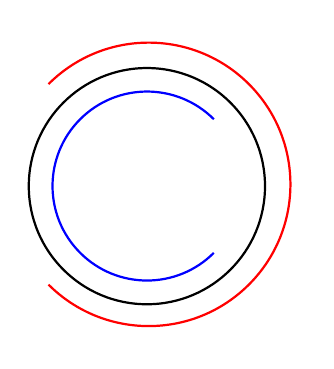
\begin{tikzpicture}[auto,scale = 1]

		\draw[thick] (0,0) circle (1.5cm);
		\draw[red,thick] (-1.25,-1.25) arc (-135:135:1.8cm);
		\draw[blue,thick] (0.85,0.85) arc (45:315:1.2cm);
		
\end{tikzpicture}
  		\end{center}
  		%\caption{}
  		%\label{}
	\end{figure}

A po-space $(X, \leq)$ is a locally partially ordered space with the atlas $\{(X,\leq)\}$. So one can define a directed path in a locally partially ordered space $X$ as a dimap from the po-space $[0,1]$ (with the usual order) to $X$. Intuitively, a directed path is a path which is locally increasing. For example, in the case of the directed circle, its directed paths are exactly the paths that turn anti-clockwise.

This category seems nicer to models looping behaviors. The counterpart is that computing colimits is hard. It is an open problem to know wether $\lpotop$ is cocomplete. In any case, the same kind of problems happen: when computing the colimit, it may be necessary to quotient more than in topological spaces and so the forgetful functor does not preserve colimits, see for example \cite{fajstrup16}.
	
	
	
	
	
	\subsection{Streams}
	
	We have seen that colimits are a problem in our search for a nice notion of directed spaces. We would like to continue this idea of defining an order locally, but this time assuring cocompleteness. The idea here is similar to free cocompletion: the ``smallest cocomplete category containing a certain category'' is its category of presheaves. We will follow the same idea with the notion of prestream \cite{krishnan09}:
	
	\begin{defi}
	A \textbf{prestream} is a topological space $X$ with a \textbf{precirculation}, i.e., a collection $(\sqsubseteq_U)_{U \in O(X)}$ where $\sqsubseteq_U$ is a preorder on the open set $U$, satisfying that for every pair of open sets, $U \subseteq V$, we have $\sqsubseteq_U \,\subseteq \,\sqsubseteq_V$. A \textbf{morphism of prestreams} $\map{f}{(X,(\sqsubseteq_U)_{U \in O(X)})}{(Y,(\preceq_V)_{V \in O(Y)})}$ is a continuous function $\map{f}{X}{Y}$ such that for open set $V$ of $Y$, for all $x, y \in f^{-1}(V)$, if $x \sqsubseteq_{f^{-1}(V)} y$ then $f(x) \preceq_V f(y)$. We note $\prestr$ the category of prestreams and morphisms of prestreams.
	\end{defi}
	
	Every po-space may be seen as a prestream: take as precirculation $\sqsubseteq_U$ the restriction of the partial order on  $U$. But we will see later that this precirculation is not necessary a good one to consider. For the case of the segment, $[0,1]$, we have another precirculation from \cite{haucourt12}: define $x \sqsubseteq_U y$ if and only if the whole segment $[x,y]$ is included in $U$. We denote this prestream by $\dirseg$. It is this structure on the segment that we will use to define directed paths in a prestream: a \textbf{directed path} in $X$ is a prestream morphism from $\dirseg$ to $X$
	
	In this category, things are much more simpler with respect to colimits:
	
	\begin{prop}
	The forgetful functor $\mathcal{F}$ from $\prestr$ to $\topo$ is topological. In particular, $\prestr$ is cocomplete and $\mathcal{F}$ preserves colimits.
	\end{prop}
	
	\begin{proof}
	Let us check the three conditions:
		\begin{itemize}
			\item $\mathcal{F}$ is faithful trivially.
			\item The order $\leq$ on the fiber corresponds to the inclusion of the precirculations and so is a partial order.
			\item Given a collection $(\map{g_i}{X}{\mathcal{F}(Y_i, \sqsubseteq^i)})_{i \in I}$ of morphisms in $\topo$, we want to construct the ``smallest'' precirculation that makes the $g_i$ morphisms of prestreams. It is defined as $x \sqsubseteq_U y$ if and only if for every $i \in I$, for every open set $V_i$ of $Y_i$ such that $U \subseteq g_i^{-1}(V_i)$, $g_i(x) \sqsubseteq^i_{V_i} g_i(y)$.
		\end{itemize}
	\end{proof}
	
	We can make the computation of the colimits more explicit. The coproduct of a family $(X_i,\sqsubseteq_i)_{i\in I}$ of prestreams is the prestream $(\bigsqcup\limits_{i\in I} X_i, \bigsqcup\limits_{i\in I} \sqsubseteq_i)$. Given a equivalence relation $\equiv$ on a prestream $(X,\sqsubseteq)$, the quotient $X/\equiv$ can be equipped with a precirculation $\preceq$ such that $\alpha \preceq_V \beta$ if and only if there is a sequence $y_1, x_2, y_2, \ldots, y_{n-1}, x_n$ of elements of $q^{-1}(V) \subseteq X$, where $\map{q}{X}{X/\equiv}$ is the quotient map, such that $q(y_1) = \alpha$, $q(x_n) = \beta$ and for all $i$, $y_i \sqsubseteq_{q^{-1}(V)} x_{i+1}$ and $x_{i+1} \equiv y_{i+1}$. Then the colimit of a small diagram $\map{D}{\D}{\prestr}$ is obtained by quotienting the coproduct of $(D(d))_{d\in\ob{\D}}$ by the smallest equivalence relation such that $(d,x) \equiv (d',D(f)(x))$ for every morphisms $\map{f}{d}{d'}$ of $\D$ and every $x \in F(d)$.
	
	There are several possible way to construct a circle in $\prestr$. The idea is to quotient the real line $\RR$ (or the segment $[0,1]$) by the equivalence relation $t \equiv t'$ if and only if $t-t'$ is an integer. Depending on the prestream  structure on $\RR$, this will give different structures on the circle. Much as the segment $[0,1]$, there are (at least) two prestream structures on $\RR$. First, the one coming from the po-space $(\RR,\leq)$, the other defined as $x \sqsubseteq_U y$ if and only if $[x,y] \subseteq U$. With the first structure, $(\RR,\leq)/\equiv$ has a trivial precirculation: with the notation of the previous paragraph, $\alpha \preceq_V \beta$ for every $\alpha$ and $\beta \in V$. Indeed, $\alpha$ is of the form $q(t)$ for some $t \in [0,1[$ and $\beta = q(t')$ for some $t' \in [0,1[$. Assume that $t \leq t'$. Then $\alpha \preceq_U \beta$. But $t' \leq t+1 \equiv t$ and so $\beta \preceq_U \alpha$. On the other side, the second structure is more interesting. In this one, $\alpha \preceq_U \beta$ if and only if the arc segment between $\alpha$ and $\beta$, turning anti-clockwise is included in $U$. This implies that the directed paths are exactly the paths that turn anti-clockwise.
	
	
	With prestreams, we define a category of ``directed spaces'' which behaves well with respects to colimits in $\topo$. The problem is that this category is too large: if we have the idea that the directed structure is defined locally, we loose the coherence of this structure, that is, the fact that if two local definitions intersect on some open neighborhood of a point, then they must coincide. To continue the parallel with free cocompletion, we consider presheaves when we would like sheaves. Following this idea, we define streams \cite{krishnan09}:
	
	\begin{defi}
	A precirculation is a \textbf{circulation} if for every family of open sets $(U_i)_{i\in I}$, $x \sqsubseteq_{\bigcup\limits_{i\in I} U_i} y$ if and only if there are a sequence $x = z_1, z_2, \ldots, z_n = y$ of points and a sequence $U_{i_1}, \ldots, U_{i_{n-1}}$ such that for every $k$, $z_k \sqsubseteq_{U_{i_k}} z_{k+1}$. We note $\str$ the full subcategory of $\prestr$ consisting of \textbf{streams}, that is prestreams whose precirculation is a circulation.
	\end{defi}
	
	This means, in particular, that if $x \sqsubseteq_U y$ then there is a chain of inequalities inside smaller open sets, as small as you want. The first structure on $\RR$ (the one from po-space) fails this condition. Indeed, take two disjoint open segments of $\RR$, say $U_1 = ]0,1[$ and $U_2 = ]2,3[$. Since $\frac{1}{2} \leq \frac{5}{2}$, $\frac{1}{2} \sqsubseteq_{U_1 \cup U_2} \frac{5}{2}$ in this structure. But there is no sequences as in the definition of a stream, because the two are disjoint. On the contrary, one can prove that the second structure is a stream.
	
	In streams, colimits initially look much harder to compute, but, in fact, not really:
	
	\begin{prop}
		The forgetful functor from $\str$ to $\topo$ is topological. Moreover, the limits in $\str$ are computed as in $\prestr$.
	\end{prop}
	
	The proof is much harder than in prestreams. See \cite{goubault14} for example for a complete proof.
	
	\subsection{Dspaces}
	
	In this subsection, we will see another point of view of ``directed spaces''. Previously, we have seen a local definition of ``directedness'' with streams and locally partially ordered spaces and then directed paths were defined by specifying a particular structure on the segment. Here, we will do things in the other way: we will specify a particular subset of paths that we will consider as ``directed'', and it is this specification that will define ``directedness''. That is the main idea of d-spaces \cite{grandis01,grandis09}:
	
	\begin{defi}
	A \textbf{d-space} is a topological space $X$ together with a subset $\dip{X}$ of $\pathsp{X}$, called the \textbf{directed paths} (or \textbf{dipaths} for short) satisfying the following:
	\begin{itemize}
		\item the constant paths are directed, i.e., for every $x \in X$, the path $c_x : t \mapsto x$ is in $\dip{X}$,
		\item dipaths are closed under concatenation, i.e., for every $\gamma_1, \gamma_2 \in \dip{X}$ with $\gamma_1(1) = \gamma_2(0)$, the path $\gamma_1\star\gamma_2$ defined as:
		\begin{align*}
			\gamma_1\star\gamma_2(t) 	&	= \gamma_1(2t) & \text{ if } t\leq \frac{1}{2}\\
      				 					&	= \gamma_2(2t-1) & \text{ if } t\geq \frac{1}{2}
		\end{align*}
		is also in $\dip{X}$,
		\item dipaths are closed under non-decreasing reparametrizations, i.e., for every $\gamma \in \dip{X}$ and every continuous and monotone function $\map{r}{[0,1]}{[0,1]}$, $\gamma\circ r \in \dip{X}$. 
	\end{itemize}
	A \textbf{dimap} between d-spaces is a continuous function $\map{f}{X}{Y}$ such that for every $\gamma \in \dip{X}$, $f\circ\gamma \in \dip{Y}$. We denote the category of d-spaces and dimaps by $\dtop$.
	\end{defi}
	
	It is very easy to add d-space structures on topological spaces. For example, on the segment $[0,1]$, one can define $\dip{[0,1]}$ as the set of non-decreasing paths, that is, continuous monotone functions. Let us note $\dirseg$ this d-space. Then for any d-space $X$, $\dip{X}$ is exactly the set of dimaps from $\dirseg$ to $X$. To define a directed circle, just define $$\dip{S^1} = \{t \mapsto e^{i\theta(t)} \mid \map{\theta}{[0,1]}{\RR} \text{ non-decreasing}\}.$$
	
	
	Given a set of paths $Q \subseteq \pathsp{X}$, there is always a smallest (for inclusion) set of paths satisfying the conditions of dipaths and containing $Q$, since $\pathsp{X}$ satisfies them and that for every collection of such sets, their intersection satisfies those axioms too. Let us note this set by $\langle Q \rangle$. It can be computed as follow:
	
	\begin{prop}
	For $\gamma_1$, \ldots, $\gamma_n$ paths with $\gamma_i(1) = \gamma_{i+1}(0)$, denote by $\gamma_1\star\ldots\star\gamma_n$ the path defined as:
	$$\gamma_1\star\ldots\star\gamma_n(t) = \gamma_{i+1}(nt-i) ~~~~~ \text{if } \frac{i}{n}\leq t \leq \frac{i+1}{n}$$
	$\langle Q \rangle$ is exactly the set of paths of the form:
	$$(\gamma_1\star\ldots\star\gamma_n)\circ r$$
	with $\gamma_i \in \{\gamma\circ q \mid \gamma \in Q, q \text{ non-decreasing reparametrization}\}\cup\{c_x \mid x \in X\}$ and $r$ a surjective non-decreasing reparametrization.
	\end{prop}
	
	But let us first prove the following lemma:
	
	\begin{lemme}
	If $Q'$ is closed under non-decreasing reparametrization, then any path $\gamma$ of the form $(\gamma_1\star\ldots\star\gamma_n)\circ r$ with $\gamma_i \in Q'$ and $r$ a non-decreasing reparametrization can also be decomposed as $(\gamma'_1\star\ldots\star\gamma'_p)\circ r'$ with $\gamma'_i \in Q'$ and $r'$ \textbf{surjective} a non-decreasing reparametrization.
	\end{lemme}
	
	\begin{proof}[Proof of the lemma]
	If $r$ is constant, let $i$ be an integer such that $\frac{i-1}{n} \leq r(0) \leq \frac{i}{n}$. Then $\gamma_i\circ(t \mapsto nr(0) - i +1) \in K$ since $K$ is closed under non-decreasing reparametrization and $(\gamma_i\circ(t \mapsto nr(0) - i +1))\circ id = (\gamma_1\star \ldots \star \gamma_n)\circ r$. Now let assume that $r$ is not constant. Let 
	$$I_0 = \{i \mid \frac{i-1}{n} \leq r(0) \leq \frac{i}{n}\}$$
	$I_0$ has one or two elements (if $r(0) = \frac{i}{n}$ or not). Let $i_0$ be the maximum of $I_0$. Since $r$ is not constant then $r(0) \neq \frac{i_0}{n}$ (a problem may have occurred if $r(0) =1$). Similarly, define $i_1$ as the minimum of $\{i \mid \frac{i-1}{n} \leq r(1) \leq \frac{i}{n}\}$. In this case, $r(1) \neq \frac{i_1-1}{n}$. Note $p = i_1 - i_0 + 1$ and $\gamma'_i = \gamma_{i_0 + i - 1}$, for $i \in \{2, \ldots, p-1\}$, $\gamma'_1 = \gamma_{i_0}\circ(t \mapsto (i_0- nr(0))t + nr(0)+1-i_0)$ and $\gamma'_p = \gamma_{i_1}\circ(t \mapsto (nr(1) +1 - i_1)t)$ (the construction is similar if $p = 1$). $\gamma'_1$ and $\gamma'_p$ belongs to $K$ since it is closed under non-decreasing reparametrization. Note $t_i = \min \{t \mid r(t) = \frac{i + i_0 - 1}{n}\}$ for all $i \in \{1, \ldots, p - 1\}$. We note $r'$ the following function:
		\begin{itemize}
			\item for $t \in [0,t_1]$, $r'(t) = \frac{n}{p(i_0-nr(0))}(r(t)-r(0))$. Remark that $r'(0) = 0$ and $r'(t_1) = \frac{1}{p}$.
			\item for $t \in [t_{p-1},1]$, $r'(t) = 1 - \frac{n}{p(nr(1) - i_1 -1)}(r(1)-r(t))$. Remark that $r'(t_{p-1}) = \frac{p-1}{p}$ and $r'(1) = 1$.
			\item for $t \in [t_i,t_{i+1}]$ for $i \in \{1,\ldots, p-2\}$, $r'(t) = \frac{n}{p}r(t) + \frac{1-i_0}{p}$. Remark that $r'(t_i) = \frac{i}{p}$ and $r'(t_{i+1}) = \frac{i+1}{p}$.
		\end{itemize}
	It is easy to check that $r'$ is a well-defined, continuous, non-decreasing and surjective. It remains to prove that $(\gamma_1\star \ldots \star \gamma_n)\circ r = (\gamma'_1\star \ldots \star \gamma'_p)\circ r'$ :
	\begin{itemize}
		\item for $t \in [0,t_1]$, $$(\gamma_1\star \ldots \star \gamma_n)\circ r(t) = \gamma_{i_0}(nr(t) +1 -i_0)$$
		and 
		\begin{eqnarray}
   			(\gamma'_1\star \ldots \star \gamma'_p)\circ r'(t) & = & \gamma'_1(pr'(t)) \nonumber \\
  			 & = & \gamma'_1(\frac{n}{i_0-nr(0)}(r(t)-r(0))) \nonumber\\
			 & = & \gamma_{i_0}(n(r(t)-r(0))+nr(0)+1 - i_0) \nonumber\\
			 & = & \gamma_{i_0}(nr(t) + 1 - i_0) \nonumber
		\end{eqnarray}
		\item for $t \in [t_{p-1},1]$, $$(\gamma_1\star \ldots \star \gamma_n)\circ r(t) = \gamma_{i_1}(nr(t) +1 -i_1)$$
		and 
		\begin{eqnarray}
   			(\gamma'_1\star \ldots \star \gamma'_p)\circ r'(t) & = & \gamma'_p(pr'(t) +1 - p) \nonumber \\
  			 & = & \gamma'_p(1 - \frac{n}{nr(1)-i_1-1}(r(1)-r(t))) \nonumber\\
			 & = & \gamma_{i_1}(nr(1)+1-i_1 - n(r(1)-r(t))) \nonumber\\
			 & = & \gamma_{i_1}(nr(t)+1-i_1) \nonumber
		\end{eqnarray}
		\item for $t \in [t_i,t_{i+1}]$, $$(\gamma_1\star \ldots \star \gamma_n)\circ r(t) = \gamma_{i_0+i}(nr(t) -i_0-i+1)$$
		and 
		\begin{eqnarray}
   			(\gamma'_1\star \ldots \star \gamma'_p)\circ r'(t) & = & \gamma'_{i+1}(pr'(t) - i) \nonumber \\
  			 & = & \gamma_{i_0+i}(nr(t)+1-i_0-i) \nonumber
		\end{eqnarray}
	\end{itemize}
	\end{proof}
	
	\begin{proof}[Proof of the proposition] Note $K$ this set of paths. Let us first prove that $K$ contains $Q$ and satisfies the axioms. Let note $Q' = \{\gamma\circ q \mid \gamma \in Q, q \text{ non-decreasing reparametrization}\}\cup\{c_x \mid x \in X\}$. Since non-decreasing reparametrizations are closed under composition, $Q'$ is closed under non-decreasing reparametrization.
	\begin{itemize}
		\item $K$ contains $Q$ (case $n =1$, $q = id$),
		\item $K$ contains constant paths (case $n = 1$),
		\item $K$ is closed under non-decreasing reparametrization by the previous lemma,
		\item Let $\gamma = (\gamma_1\star\ldots\star\gamma_n)\circ r$ and $\gamma' = (\gamma'_1\star\ldots\star\gamma'_m)\circ r'$ be two elements of $K$, such that $\gamma(1) = \gamma'(0)$. Since $r$ and $r'$ are surjective:
		$$\gamma\star\gamma' = (\gamma_1\star\ldots\star\gamma_n\star\gamma'_1\star\ldots\star\gamma'_m)\circ (r\star r')$$
		with $r\star r'$ surjective. Consequently, $\gamma\star\gamma' \in K$. 
	\end{itemize}
	
	Now let us prove that this is the smallest one, that is, given such a set $K'$, then $K \subseteq K'$. Let $\gamma = (\gamma_1\star\ldots\star\gamma_n)\circ r \in K$. We want to prove that $\gamma \in K'$. Since $K'$ is closed under non-decreasing reparametrization, it is enough to prove that $\gamma_1\star\ldots\star\gamma_n \in K'$. $\gamma_1\star\ldots\star\gamma_n$ is equal up to non-decreasing reparametrization to $(\gamma_1 \star (\gamma_2 \star (\ldots \star (\gamma_{n-1}\star\gamma_n)\ldots)))$ and since $K'$ is closed under non-decreasing reparametrization and concatenation, it is enough to prove that $\gamma_i \in K'$, which is true since $K'$ contains constant paths, $Q$ and is closed under non-decreasing reparametrizations.
	\end{proof}
	
	\begin{prop}
	$\dtop$ is cocomplete.
	\end{prop}
	
	Indeed, given a small diagram $\map{D}{\D}{\dtop}$, the colimit of $D$ is computed as follow. Form first the colimit in $\topo$, that is, the space:
	
	$$X = \bigsqcup\limits_{d\in\ob{\D}} D(d) / \sim$$
	
\noindent where $\sim$ is the smallest equivalence relation such that $(d,x) \sim (d',D(f)(x))$ for every morphism $\map{f}{d}{d'}$. Denote the quotient map by $\map{p_d}{D(d)}{X}$. Define $\dip{X}$ as $\langle Q \rangle$ where:
	$$Q = \{p_d\circ\gamma \mid d\in \ob{\D}, \gamma \in \dip{D(d)}\}.$$
	
	In particular, we observe that the forgetful functor from $\dtop$ to $\topo$ preserves colimits. Actually, we have better:
	
	\begin{prop}
	This forgetful functor is topological.
	\end{prop}
	
	\begin{proof}
	Let us prove the three axioms:
	\begin{itemize}
		\item Faithfulness is trivial.
		\item The order on each fiber corresponds to the inclusion of sets of dipaths, and so is a partial order.
		\item Assume given a collection of morphisms $(\map{g_i}{X}{F(Y_i)})_{i\in I}$. Define $\dip{X}$ as the set:
		$$\{\gamma \in \pathsp{X} \mid \forall i, \, g_i\circ\gamma \in \dip{Y_i}\}.$$
	\end{itemize}
	\end{proof}
	
	\subsection{Comparison}
	
	For every stream $(X,\sqsubseteq)$, the directed paths, that is, the morphisms of prestreams from $\dirseg$ to $X$ satisfies the conditions of dipaths of a d-space. This extends to a functor $\map{S}{\str}{\dtop}$. Reciprocally, from a d-space $X$, one can define a circulation $\sqsubseteq$ such that $x\sqsubseteq_U y$ if and only if there is a dipath $\gamma \in \dip{X}$ with $\gamma(0) = x$, $\gamma(1) = y$ and the image of $\gamma$ is included in $U$. This extends to a functor $\map{D}{\dtop}{\str}$.
	
	As observed in \cite{haucourt12}, $S$ is left adjoint to $D$, $D\circ S\circ D = D$ and $S\circ D\circ S = S$. This implies in particular that if $\hstr$ denotes the full subcategory of $\str$ of streams which are in the image of $D$ and $\cdtop$ denote the full subcategory of $\dtop$ of d-spaces which are in the image of $S$, then $S$ and $D$ restrict to functors $\map{\bar{S}}{\cdtop}{\hstr}$ and $\map{\bar{D}}{\hstr}{\dtop}$ which form an equivalence of categories. 
	
	In the literature, those streams (resp. d-spaces) have been considered. First, streams in $\hstr$ are called \textbf{Haucourt streams} in \cite{goubault14}. They can be characterized by the following: a Haucourt stream is a stream $(X,\sqsubseteq)$ whose circulation satisfies that for every open set $U$ and $x, y \in U$, $x \sqsubseteq_U y$ if and only if there is a directed paths (that is a prestream morphism from $\dirseg$ to $X$) with $\gamma(0) = x$, $\gamma(1) = y$ and the image of $\gamma$ is included in $U$. Let us prove this statement. 
	
	We first prove that streams in the image of $D$ are Haucourt. Let $X$ be a d-space. $D(X)$ is of the form $(X,\sqsubseteq)$. Let $x \subseteq_U y$, i.e., there is a dipath $\gamma \in \dip{X}$ from $x$ to $y$ with image included in $U$. We prove that this $\gamma$ is a directed path in $(X,\sqsubseteq)$, that is, a prestream morphism from $\dirseg$ to $(X,\sqsubseteq)$. So let $V$ be a open set of $X$ and $[t,t'] \subseteq \gamma^{-1}(V)$. We must prove that $\gamma(t) \sqsubseteq_V \gamma(t')$, that is, there is a dipath $\gamma'$ from $\gamma(t)$ to $\gamma(t')$ with image included in $V$. Define the non-decreasing reparametrization $r(u) = (t' - t).u + t$. Then $\gamma' = \gamma\circ r$ is such a dipath. Reciprocally, let us assume there is a prestream morphism $\map{\gamma}{\dirseg}{(X,\sqsubseteq)}$ from $x$ to $y$ with image included in $U$. We must construct a dipath $\gamma'$ (which will not necessarily be $\gamma$) from $x$ to $y$ with image included in $U$. Since the image of $\gamma$ is included in $U$, $[0,1] \subseteq \gamma^{-1}(U)$. So since $\gamma$ is a prestream morphism $x = \gamma(0) \sqsubseteq_U \gamma(0) = y$, which provides the desired dipath.
	
	We prove now that every Haucourt stream is in the image of $D$, more precisely, that for every Haucourt stream $(X,\sqsubseteq)$, $D\circ S(X,\sqsubseteq) = (X,\subseteq)$. Since $S$ and $D$ do not change the underlying space, we must prove that if $\preceq$ is the circulation of $D\circ S(X,\sqsubseteq)$ then $\preceq \, = \, \sqsubseteq$. $\preceq$ is defined as follow: $x \preceq_U y$ if and only if there is a directed path in $(X,\sqsubseteq)$ from $x$ to $y$ with image included in $U$, which is equivalent to $x \sqsubseteq_U y$ because $(X,\sqsubseteq)$ is Haucourt.
	
	Secondly, d-spaces in $\cdtop$ are called \textbf{complete d-spaces} in \cite{ziemianski12}. They are defined as follow. We call \textbf{weak dipaths of a d-space $X$} a path $\gamma$ of $X$ such that for every open set $V$, for every $t \leq t'$ such that $[t,t'] \subseteq \gamma^{-1}(V)$, there is a dipath $\gamma' \in \dip{X}$ from $\gamma(t)$ to $\gamma(t')$ with image included in $V$. Weak dipaths satisfy the axioms of dipaths in d-spaces and we denote the d-space whose dipaths are weak dipaths by $\bar{X}$. Another way to formulate this is that $\bar{X} = S\circ D(X)$. We say that a d-space is \textbf{complete} if and only if $X = \bar{X}$ or, equivalently, if and only if every weak dipath is a dipath. Since $\bar{X} = S\circ D(X)$, then a complete d-space is in the image of $S$. Reciprocally, let $(X,\sqsubseteq)$ be a stream. Let us prove that $S(X)$ is complete, that is, every weak dipath $\gamma$ is a directed path. Let $V$ be an open set of $X$ and $t \leq t'$ with $[t,t'] \subseteq \gamma^{-1}(V)$. Since $\gamma$ is a weak dipath, there is a directed path $\gamma'$ from $\gamma(t)$ to $\gamma(t')$ with image included in $V$. The latter says that $[0,1] \subseteq \gamma'^{-1}(V)$ and since $\gamma'$ is stream morphism this implies that $\gamma'(0) \sqsubseteq_V \gamma'(1)$, that is, $\gamma(t) \sqsubseteq_V \gamma(t')$.



\section{Geometric view of true concurrency}
\label{sec:geovi}

Now that we have seen an overview of the possible way of expressing directedness, we choose to use d-spaces from now.  Fix such a d-space $X$ with dipaths $\dip{X}$. We denote by $\dipp{X}{x}{y}$ the set of dipaths from $x$ to $y$. $\dip{X}$ and $\dipp{X}{x}{y}$ can be equipped with the subspace topology from $\pathsp{X}$, that is why we will call them \textbf{dipath spaces}.

Recall that we have defined homotopy as a path in the space of paths. We can do the same here: we call \textbf{dihomotopy} \cite{fajstrup16} between two dipaths $\gamma, \gamma'$ from $x$ to $y$ a continuous function $$\map{H}{[0,1]}{\dipp{X}{x}{y}}$$ such that $H(0) = \gamma$ and $H(1) = \gamma'$. In this case, we say that $\gamma$ and $\gamma'$ are \textbf{dihomotopic}, and we denote by $[\gamma]$ the equivalence class of $\gamma$.

The idea is, intuitively, that two dipaths are dihomotopic if we can continuously deform one into the other while staying a dipath during the deformation. Let illustrate this on a example. Consider the following d-space.

	\begin{figure}[H]
		\begin{center}
    			\input{images/Geomod/square}
  		\end{center}
  		%\caption{}
  		%\label{}
	\end{figure}

\noindent It consists of a square $[0,1]^2$ (in white) from which we have carved out a smaller square $[\frac{1}{3},\frac{2}{3}]^2$ (in gray), equipped with the subspace topology from $\RR^2$. Observe that it is the geometric realization of the program $P_1.V_1\parallel P_1.V_1$, or of the program $U\parallel S$. The dipaths are the paths that are monotone component-wise. If we consider the following two dipaths, on the left:

	\begin{figure}[H]
		\begin{center}
    			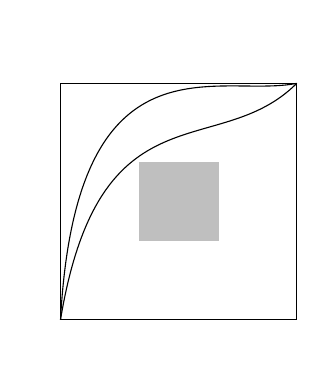
\begin{tikzpicture}[auto,scale = 1]
		\node at (-0.3,-0.3) {};
		\draw (0,0) rectangle (3,3);
		\draw [fill = gray!50,draw = gray!50] (1,1) rectangle (2,2);
		\draw (0,0) .. controls (0.5,3) and (2,2) .. (3,3);
		\draw (0,0) .. controls (0.2,3.7) and (2,2.8) .. (3,3);
\end{tikzpicture}
\begin{tikzpicture}[auto,scale = 1.5]
	\draw[draw = white] (0,0) rectangle (1,1);
\end{tikzpicture}
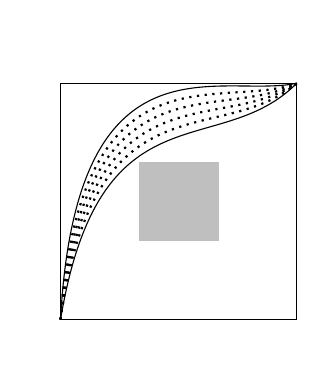
\begin{tikzpicture}[auto,scale = 1]
		\node at (-0.3,-0.3) {};
		\draw (0,0) rectangle (3,3);
		\draw [fill = gray!50,draw = gray!50] (1,1) rectangle (2,2);
		\draw (0,0) .. controls (0.5,3) and (2,2) .. (3,3);
		\draw[dotted,thick] (0,0) .. controls ({0.5*(1-0.2)+0.2*0.2},{3*(1-0.2)+3.7*0.2}) and (2,{2*(1-0.2)+2.8*0.2}) .. (3,3);
		\draw[dotted,thick] (0,0) .. controls ({0.5*(1-0.4)+0.2*0.4},{3*(1-0.4)+3.7*0.4}) and (2,{2*(1-0.4)+2.8*0.4}) .. (3,3);
		\draw[dotted,thick] (0,0) .. controls ({0.5*(1-0.6)+0.2*0.6},{3*(1-0.6)+3.7*0.6}) and (2,{2*(1-0.6)+2.8*0.6}) .. (3,3);
		\draw[dotted,thick] (0,0) .. controls ({0.5*(1-0.8)+0.2*0.8},{3*(1-0.8)+3.7*0.8}) and (2,{2*(1-0.8)+2.8*0.8}) .. (3,3);
		\draw (0,0) .. controls (0.2,3.7) and (2,2.8) .. (3,3);
\end{tikzpicture}
  		\end{center}
  		\caption{(Di)homotopic dipaths}
  		%\label{}
	\end{figure}

\noindent whose images are depicted on the space, these two dipaths are dihomotopic since we can continuously deform one into the other while staying a dipath as depicted on the right. On the other hand, if we consider the following two dipaths, on the left:

	\begin{figure}[H]
		\begin{center}
    			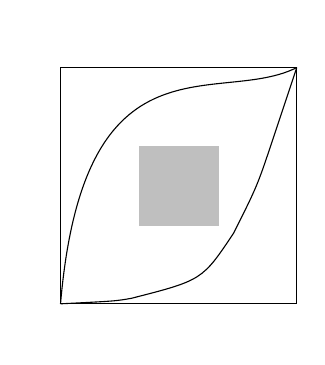
\begin{tikzpicture}[auto,scale = 1]
		\node at (-0.3,-0.3) {};
		\draw (0,0) rectangle (3,3);
		\draw [fill = gray!50,draw = gray!50] (1,1) rectangle (2,2);
		\draw (0,0) .. controls (0.3,3.5) and (2,2.5) .. (3,3);
		\draw (0,0) .. controls (0.7,0.035) .. (0.9,0.07) .. controls (1.8,0.3) .. (2.2,0.9) .. controls (2.5,1.5) ..  (2.7,2.1) .. controls (3,3) .. (3,3);
\end{tikzpicture}
\begin{tikzpicture}
		\draw[color = white] (0,0) rectangle (1,1);
\end{tikzpicture}
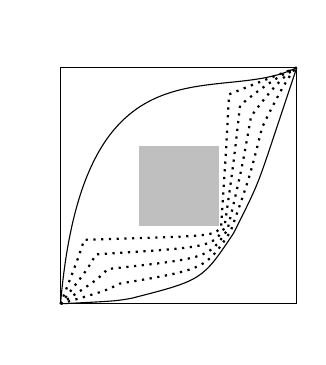
\begin{tikzpicture}[auto,scale = 1]
		\node at (-0.3,-0.3) {};
		\draw (0,0) rectangle (3,3);
		\draw [fill = gray!50,draw = gray!50] (1,1) rectangle (2,2);
		\draw (0,0) .. controls (0.3,3.5) and (2,2.5) .. (3,3);
		\draw (0,0) .. controls (0.7,0.035) .. (0.9,0.07) .. controls (1.8,0.3) .. (2.2,0.9) .. controls (2.5,1.5) ..  (2.7,2.1) .. controls (3,3) .. (3,3);
		\draw[dotted,thick] (0,0) .. controls ({0.7*(1-0.2)+0.1*0.2},{0.035*(1-0.2)+0.7*0.2}) .. ({0.9*(1-0.2) + 0.15*0.2},{0.07*(1-0.2)+0.2}) 
			.. controls ({1.8*(1-0.2)+2*0.2},{0.3*(1-0.2)+0.2}) .. ({2.2*(1-0.2)+2*0.2},{0.9*(1-0.2)+0.2})
			.. controls ({2.5*(1-0.2)+2*0.2},{1.5*(1-0.2)+2*0.2}) .. ({2.7*(1-0.2)+2*0.2},{2.1*(1-0.2)+2.8*0.2})
			.. controls ({3*(1-0.2)+2.55*0.2},{3*(1-0.2)+2.83*0.2}) and (3,3) .. (3,3);
		\draw[dotted,thick] (0,0) .. controls ({0.7*(1-0.4)+0.1*0.4},{0.035*(1-0.4)+0.7*0.4}) .. ({0.9*(1-0.4) + 0.15*0.4},{0.07*(1-0.4)+0.4}) 
			.. controls ({1.8*(1-0.4)+2*0.4},{0.3*(1-0.4)+0.4}) .. ({2.2*(1-0.4)+2*0.4},{0.9*(1-0.4)+0.4})
			.. controls ({2.5*(1-0.4)+2*0.4},{1.5*(1-0.4)+2*0.4}) .. ({2.7*(1-0.4)+2*0.4},{2.1*(1-0.4)+2.8*0.4})
			.. controls ({3*(1-0.4)+2.55*0.4},{3*(1-0.4)+2.83*0.4}) and (3,3) .. (3,3);
		\draw[dotted,thick] (0,0) .. controls ({0.7*(1-0.6)+0.1*0.6},{0.035*(1-0.6)+0.7*0.6}) .. ({0.9*(1-0.6) + 0.15*0.6},{0.07*(1-0.6)+0.6}) 
			.. controls ({1.8*(1-0.6)+2*0.6},{0.3*(1-0.6)+0.6}) .. ({2.2*(1-0.6)+2*0.6},{0.9*(1-0.6)+0.6})
			.. controls ({2.5*(1-0.6)+2*0.6},{1.5*(1-0.6)+2*0.6}) .. ({2.7*(1-0.6)+2*0.6},{2.1*(1-0.6)+2.8*0.6})
			.. controls ({3*(1-0.6)+2.55*0.6},{3*(1-0.6)+2.83*0.6}) and (3,3) .. (3,3);
		\draw[dotted,thick] (0,0) .. controls ({0.7*(1-0.8)+0.1*0.8},{0.035*(1-0.8)+0.7*0.8}) .. ({0.9*(1-0.8) + 0.15*0.8},{0.07*(1-0.8)+0.8}) 
			.. controls ({1.8*(1-0.8)+2*0.8},{0.3*(1-0.8)+0.8}) .. ({2.2*(1-0.8)+2*0.8},{0.9*(1-0.8)+0.8})
			.. controls ({2.5*(1-0.8)+2*0.8},{1.5*(1-0.8)+2*0.8}) .. ({2.7*(1-0.8)+2*0.8},{2.1*(1-0.8)+2.8*0.8})
			.. controls ({3*(1-0.8)+2.55*0.8},{3*(1-0.8)+2.83*0.8}) and (3,3) .. (3,3);
\end{tikzpicture}
  		\end{center}
  		\caption{Non-(di)homotopic dipaths}
  		%\label{}
	\end{figure}

\noindent those two dipaths are not dihomotopic because if we want to continuously deform one into the other, we would be blocked by the hole.


At the beginning of the section, we have seen two ways of defining homotopy: either as a function $\map{H}{[0,1]\times [0,1]}{X}$, or as a function $\map{H}{[0,1]}{\pathspp{X}{x}{y}}$. We choose to extend the second definition to d-spaces but we could have done the same with the first. The main point comes from the possible directed structures with which one can equip the segment. We have seen the directed segment $\dirseg$ whose dipath are monotone paths. Symmetrically, $\dirsegrev$ is the d-space whose dipaths are antitonic paths. Since the set of d-space structures on a topological space is a complete lattice, there is a smallest d-space structure that contains $\dirseg$ and $\dirsegrev$, that we denote by $\revseg$. to be more explicit, the dipaths of $\revseg$ are the paths that only have a finite number of changes of monoticity, or equivalently, that are finite concatenations of monotonic and antitonic paths. But there are two others structures on the segment coming from the adjunctions of the forgetful functor from d-spaces to topological spaces. Given a topological space $X$, one can always define two directed structures on it:
\begin{itemize}
	\item $\overline{X}$ whose dipaths are constant paths. This is the smallest (for inclusion) possible structure on a topological space.
	\item $\overleftrightarrow{X}$ whose dipaths are all the paths. This is the largest possible structure on a topological space.
\end{itemize}
It has to be noticed that $\revseg$ and $\overleftrightarrow{[0,1]}$ do not coincide, since there are paths that have an infinite number of changes of monoticity (for example, $t \mapsto t\sin(\frac{1}{t})$).
In the following, we will consider topological spaces as d-spaces by implicitly using the structure $\overleftrightarrow{X}$. The other structure also has its own interest: a dihomotopy defined as a continuous function $\map{H}{[0,1]}{\dipp{X}{x}{y}}$ is the same as a dimap $\map{H}{\overline{[0,1]}\times\dirseg}{X}$ with some boundary conditions. One could argue: why this choice ? The point is that we are interested in continuous deformation of dipaths (executions) such that during the deformation we always have a dipath (execution), but we do not care about directedness of the deformation. Some authors (see \cite{grandis09}, for example) chose to use $\dirseg$ instead of $\overline{[0,1]}$. Using the definition as a map from $[0,1]$ to $\dipp{X}{x}{y}$, using $\dirseg$ means that we consider dihomotopies as dipaths in the (suitable) d-space of dipaths. It does make a difference in general, in particular, if one has in mind that topological spaces are $\infty$-groupoids, considering $\dip{X}$ as a topological space means that, intuitively (we will come to this more precisely later), $X$ can be seen as an $(\infty,1)$-category, while seeing $\dip{X}$ as a d-space means that $X$ can be seen as an $(\infty,\infty)$-category.


A dipath being also a path, one may be wondering how homotopy between dipaths and dihomotopy can be compared. In the previous example, these two equivalence relations on dipaths coincide: the fact that, during the deformation, one must stay a dipath is not important. It is a general behavior for simple spaces (see \cite{goubault16}, in the case of non-positively curved spaces). But there are space for which homotopy and dihomotopy are different, and this is important !

Let us illustrate this on the following example, called the \textbf{matchbox}, from \cite{fahrenberg03}:

	\begin{figure}[H]
		\begin{center}
    			\scalebox{1}{\input{images/GeoMod/matchbox.pdf_t}
			\quad\quad
    			\input{images/GeoMod/matchhom}}
  		\end{center}
  		\caption{The matchbox and some homotopic behavior}
  		%\label{}
	\end{figure}

\noindent This d-space is constructed as follow. Consider the topological cube $\Box_3$, i.e., the set of triples $(t_1,t_2,t_3)$ such that $t_i \in [0,1]$. The matchbox $\matchbox$ is then the sub-space of $\Box_3$ whose points are triples $(t_1,t_2,t_3)$ with $t_1 \in \{0,1\}$ or $t_2 \in \{0,1\}$ or $t_3 = 1$. Geometrically, $\matchbox$ is a hollow cube whose lower face has been cut. $\Box_3$ can be equipped with a structure of po-space by the product ordering, and so of a d-space structure whose dipaths are monotonic paths. $\matchbox$ has two particular dipaths depicted in blue and green on the above right picture. These two dipaths are homotopic, a homotopy is drawn of the right. But during this deformation, one must cross the upper face and at this point, the path must go down and so is not monotone. Consequently, this homotopy is not a dihomotopy. More generally, any homotopy must intersect the upper face and so cannot be a dihomotopy. Those dipaths are then not dihomotopic.

We choose to present this example because it is a very simple space to describe, but the problem also occur for geometric realizations of concurrent programs. Consider for example the program $P_1.V_1\parallel P_1.V_1 \parallel P_1.V_1$ with $\nu_1 = 2$. Its geometric realization is the following, on the left, a face view is depicted in the middle, and a side view on the right:
	\begin{figure}[H]
		\begin{center}
    			\begin{tikzpicture}[thick,scale=3]

    \draw[blue,very thick] (0.35,0.2) .. controls (0.9,0.3) and (0.9,0.5) .. (0.85,1.15);
    \coordinate (A1) at (0, 0);
    \coordinate (A2) at (0, 1);
    \coordinate (A3) at (1, 1);
    \coordinate (A4) at (1, 0);
    \coordinate (B1) at (0.3, 0.3);
    \coordinate (B2) at (0.3, 1.3);
    \coordinate (B3) at (1.3, 1.3);
    \coordinate (B4) at (1.3, 0.3);



    \draw[dashed] (A1) -- (B1);
    \draw[dashed] (B1) -- (B2);
    \draw[very thick] (A2) -- (B2);
    \draw[very thick] (B2) -- (B3);
    \draw[very thick] (A3) -- (B3);
    \draw[very thick] (A4) -- (B4);
    \draw[very thick] (B4) -- (B3);
    \draw[dashed] (B1) -- (B4);
    
    \coordinate (A13) at (0.33, 0.33);
    \coordinate (A23) at (0.33, 0.83);
    \coordinate (A33) at (0.83, 0.83);
    \coordinate (A43) at (0.83, 0.33);
    \coordinate (B13) at (0.48, 0.48);
    \coordinate (B23) at (0.48, 0.98);
    \coordinate (B33) at (0.98, 0.98);
    \coordinate (B43) at (0.98, 0.48);

    \draw[very thick,color = gray] (A13) -- (A23);
    \draw[very thick,color = gray] (A23) -- (A33);
    \draw[very thick,color = gray] (A33) -- (A43);
    \draw[very thick,color = gray] (A43) -- (A13);

    \draw[dashed,color = gray] (A13) -- (B13);
    \draw[dashed,color = gray] (B13) -- (B23);
    \draw[very thick,color = gray] (A23) -- (B23);
    \draw[very thick,color = gray] (B23) -- (B33);
    \draw[very thick,color = gray] (A33) -- (B33);
    \draw[very thick,color = gray] (A43) -- (B43);
    \draw[very thick,color = gray] (B43) -- (B33);
    \draw[dashed,color = gray] (B13) -- (B43);
    
    \draw[fill=gray,opacity = 0.4] (A13) -- (B13) -- (B43) -- (A43);
    \draw[fill=gray,opacity = 0.4] (A13) -- (A23) -- (A33) -- (A43);
    \draw[fill=gray,opacity = 0.4] (A13) -- (A23) -- (B23) -- (B13);
    \draw[fill=gray,opacity = 0.4] (B13) -- (B23) -- (B33) -- (B43);
    \draw[fill=gray,opacity = 0.4] (A33) -- (B33) -- (B43) -- (A43);
    \draw[fill=gray,opacity = 0.4] (A23) -- (B23) -- (B33) -- (A33);
    
    \draw[blackorkgreen,very thick] (0.35,0.2) .. controls (0.5,0.75) and (0.8,1.1) .. (0.85,1.15);
\draw[red,very thick] (0.35,0.2) .. controls (1.6,0.2) and (1.0,1.3) .. (0.85,1.15);
    
    \draw[very thick] (A1) -- (A2);
    \draw[very thick] (A2) -- (A3);
    \draw[very thick] (A3) -- (A4);
    \draw[very thick] (A4) -- (A1);
    
\end{tikzpicture}
\begin{tikzpicture}
\draw[color = white] (0,-1) rectangle (1.2,-1.1);
\end{tikzpicture}
\begin{tikzpicture}[auto,scale = 1]
\draw (0,0) rectangle (3,3);
\draw[blue,very thick] (1.2,0.7) .. controls (1.8,0.8) and (1.7,1.1) .. (1.8,2.3);
\draw [fill = gray!50,draw = gray!50] (1,1) rectangle (2,2);
\draw[blackorkgreen,very thick] (1.2,0.7) .. controls (1.4,1.5) and (1.6,2.1) .. (1.8,2.3);
\draw[red,very thick] (1.2,0.7) .. controls (3,0.7) and (2.4,2.7) .. (1.8,2.3);
\node (uf) at (3.5,1) {};
\end{tikzpicture}
\begin{tikzpicture}
\draw[color = white] (0,-1) rectangle (1.5,-1.1);
\end{tikzpicture}
\begin{tikzpicture}[auto,scale = 1]
\draw (0,0) rectangle (3,3);
\draw [fill = gray!50,draw = gray!50] (1,1) rectangle (2,2);
\draw[blackorkgreen,very thick] (0.7,0.7) .. controls (0.75,2.4) and (0.9,2.25) .. (2.3,2.3);
\draw[blue,very thick] (0.7,0.7) .. controls (2.4,0.75) and (2.25,0.9) .. (2.3,2.3);
\draw[red,very thick] (0.7,0.7) -- (2.3,2.3);
\node (uf) at (3.5,1) {};
\end{tikzpicture}








  		\end{center}
	\end{figure}
More precisely, it is the space $[0,1]\times [0,1]\times [0,1] \backslash \left[\frac{1}{3},\frac{2}{3}\right] \times \left[\frac{1}{3},\frac{2}{3}\right] \times \left[\frac{1}{3},\frac{2}{3}\right]$. Consider as dipaths the monotone paths. The blue and green paths are homotopic just turn around the hole. But they are not dihomotopic since a homotopy must go through a path similar to the red one depicted above, which cannot be a dipath.


Actually, the things are even trickier. If you extend the blue and green dipaths in the matchbox with the red dipaths as follow:

	\begin{figure}[H]
		\begin{center}
    			 \begin{tikzpicture}[auto,scale = 1]
 		\node at (-2,-0.5) {};
		\coordinate (A) at (0,0);
		\coordinate (B) at (2,0.9);
		\coordinate (C) at (-1.3,1.8);
		\coordinate (D) at (0.7,2.6);
		\coordinate (A') at (0,1);
		\coordinate (B') at (2,1.9);
		\coordinate (C') at (-1.3,2.8);
		\coordinate (D') at (0.7,3.6);
		\draw (B) -- (B');
		\draw (A') -- (B');
		\draw (C) -- (C');
		\draw (A') -- (C');
		\draw (B') -- (D');
		\draw (C') -- (D');
		\draw [fill = gray,draw = black,opacity = 0.2] (A) -- (B) -- (B') -- (A') -- (A);
		\draw [fill = gray,draw = black,opacity = 0.2] (A) -- (C) -- (C') -- (A') -- (A);
		\draw [fill = gray,draw = black,opacity = 0.2] (A') -- (B') -- (D') -- (C') -- (A');
		\draw[blackorkgreen,very thick] (A) -- (B);
		\draw[blue,very thick] (A) -- (C);
		\draw[blackorkgreen,very thick] (B) -- (D);
		\draw[blue,very thick] (C) -- (D);
		\draw[red, very thick] (D) -- (D');
\end{tikzpicture}

  		\end{center}
  		\caption{Non-cancellative behavior in the matchbox}
  		\label{fig:matchdihom}
	\end{figure}
\vspace{-0.5cm	}
\noindent the extended dipaths are dihomotopic. This means that dihomotopies may have non-cancellative behaviors: non-dihomotopic dipaths may become dihomotopic after concatenation. This kind of behavior cannot occur with homotopy in topological spaces. Indeed, a path is always invertible up to homotopy: given a path $\map{\gamma}{[0,1]}{X}$, the path $\gamma^{-1}$ which maps $t$ to $\gamma(1-t)$  satisfy that $\gamma\star\gamma^{-1}$ and $\gamma^{-1}\star\gamma$ are homotopic to constant paths. So, since homotopy is preserved by concatenation, if $\tau\star\gamma$ and $\rho\star\gamma$ are homotopic then $\tau$ is homotopic to $\tau\star\gamma\star\gamma^{-1}$, which is homotopic to $\rho\star\gamma\star\gamma^{-1}$, itself homotopic to $\rho$. 

All those data can be summarized in one structure, the \textbf{fundamental category} \cite{brown06}. Given a topological space $X$, the fundamental category $\pi_1(X)$ is the category whose:
\begin{itemize}
	\item objects are points of $X$,
	\item morphisms from $x$ to $y$ are paths from $x$ to $y$ modulo homotopy,
	\item composition $[\gamma]\circ[\rho]$ is given by $[\rho\star\gamma]$,
	\item identities are equivalence classes of constant paths $[c_x]$.
\end{itemize}

\noindent This category is well defined: 
\begin{itemize}
	\item the composition does not depend on the representative elements used: if $H$ is a homotopy between $\gamma$ and $\gamma'$, and $H'$ between $\rho$ and $\rho'$ then $H\star H'$ defined as $t\mapsto H(t)\star H'(t)$ is a homotopy between $\gamma\star\rho$ and $\gamma'\star\rho'$.
	\item the composition is associative: concatenation is not associative but $(\gamma_1\star\gamma_2)\star\gamma_3$ is homotopic to $\gamma_1\star(\gamma_2\star\gamma_3)$. Actually, there is a reparametrization $r$ such that $(\gamma_1\star(\gamma_2\star\gamma_3))\circ r = (\gamma_1\star\gamma_2)\star\gamma_3$.
	\begin{figure}[H]
		\begin{center}
    			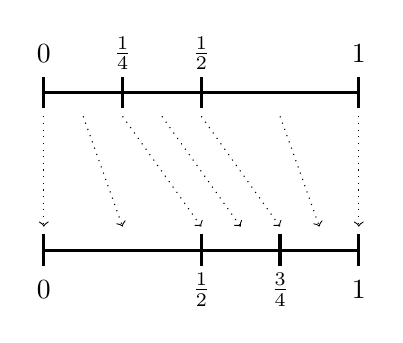
\begin{tikzpicture}[auto,scale = 1]
	\draw[very thick] (0,0) -- (4,0);
	\draw[very thick] (0,-2) -- (4,-2);
	\draw[very thick] (0,-0.2) -- (0,0.2);
	\draw[very thick] (1,-0.2) -- (1,0.2);
	\draw[very thick] (2,-0.2) -- (2,0.2);
	\draw[very thick] (4,-0.2) -- (4,0.2);
	\draw[very thick] (0,-2.2) -- (0,-1.8);
	\draw[very thick] (2,-2.2) -- (2,-1.8);
	\draw[very thick] (3,-2.2) -- (3,-1.8);
	\draw[very thick] (4,-2.2) -- (4,-1.8);
	\node at (0,0.5) {$0$};
	\node at (1,0.5) {$\frac{1}{4}$};
	\node at (2,0.5) {$\frac{1}{2}$};
	\node at (4,0.5) {$1$};
	\node at (0,-2.5) {$0$};
	\node at (2,-2.5) {$\frac{1}{2}$};
	\node at (3,-2.5) {$\frac{3}{4}$};
	\node at (4,-2.5) {$1$};
	\draw[dotted, ->] (0,-0.3) -- (0,-1.7);
	\draw[dotted, ->] (1,-0.3) -- (2,-1.7);
	\draw[dotted, ->] (2,-0.3) -- (3,-1.7);
	\draw[dotted, ->] (4,-0.3) -- (4,-1.7);
	\draw[dotted, ->] (0.5,-0.3) -- (1,-1.7);
	\draw[dotted, ->] (1.5,-0.3) -- (2.5,-1.7);
	\draw[dotted, ->] (3,-0.3) -- (3.5,-1.7);
\end{tikzpicture}
	
  		\end{center}
  		%\caption{}
  		%\label{}
	\end{figure}
	\item the constant paths are neutral elements for concatenation modulo dihomotopy: $c_x\star\gamma$ and $\gamma\star c_y$ are both homotopic to $\gamma$. Actually, there are reparametrizations as previously.
	\begin{figure}[H]
		\begin{center}
    			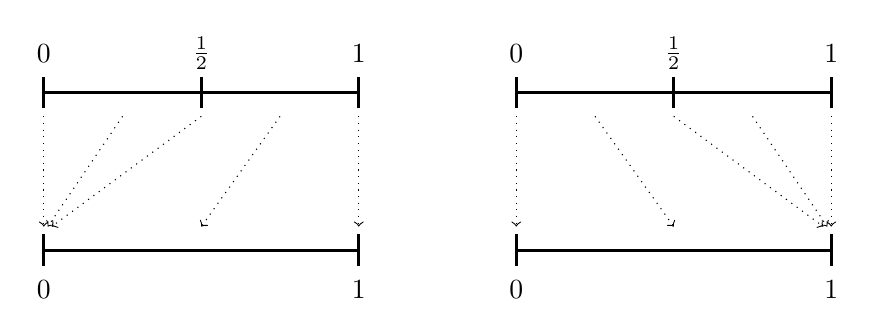
\begin{tikzpicture}[auto,scale = 1]
	\draw[very thick] (0,0) -- (4,0);
	\draw[very thick] (0,-2) -- (4,-2);
	\draw[very thick] (0,-0.2) -- (0,0.2);
	\draw[very thick] (2,-0.2) -- (2,0.2);
	\draw[very thick] (4,-0.2) -- (4,0.2);
	\draw[very thick] (0,-2.2) -- (0,-1.8);
	\draw[very thick] (4,-2.2) -- (4,-1.8);
	\node at (0,0.5) {$0$};
	\node at (2,0.5) {$\frac{1}{2}$};
	\node at (4,0.5) {$1$};
	\node at (0,-2.5) {$0$};
	\node at (4,-2.5) {$1$};
	\draw[dotted, ->] (0,-0.3) -- (0,-1.7);
	\draw[dotted, ->] (2,-0.3) -- (0.1,-1.7);
	\draw[dotted, ->] (4,-0.3) -- (4,-1.7);
	\draw[dotted, ->] (1,-0.3) -- (0.05,-1.7);
	\draw[dotted, ->] (3,-0.3) -- (2,-1.7);
	
	\draw[very thick] (6,0) -- (10,0);
	\draw[very thick] (6,-2) -- (10,-2);
	\draw[very thick] (6,-0.2) -- (6,0.2);
	\draw[very thick] (8,-0.2) -- (8,0.2);
	\draw[very thick] (10,-0.2) -- (10,0.2);
	\draw[very thick] (6,-2.2) -- (6,-1.8);
	\draw[very thick] (10,-2.2) -- (10,-1.8);
	\node at (6,0.5) {$0$};
	\node at (8,0.5) {$\frac{1}{2}$};
	\node at (10,0.5) {$1$};
	\node at (6,-2.5) {$0$};
	\node at (10,-2.5) {$1$};
	\draw[dotted, ->] (6,-0.3) -- (6,-1.7);
	\draw[dotted, ->] (8,-0.3) -- (9.9,-1.7);
	\draw[dotted, ->] (10,-0.3) -- (10,-1.7);
	\draw[dotted, ->] (7,-0.3) -- (8,-1.7);
	\draw[dotted, ->] (9,-0.3) -- (9.95,-1.7);
\end{tikzpicture}
	
  		\end{center}
  		%\caption{}
  		%\label{}
	\end{figure}
\end{itemize}

The existence of an inverse path modulo homotopy implies that this category is always a groupoid, that is, a category such that every morphism is an isomorphism. That is why we talk about the \textbf{fundamental groupoid} of $X$. A groupoid is in particular left and right cancellative, that is, if $f \circ g = f\circ h$ then $g = h$, and symmetrically, as observed earlier on paths modulo homotopy.

This construction extends to a functor $\map{\pi_1}{\topo}{\grpd}$, where $\grpd$ is the category of small groupoids and functors. For a continuous map $\map{f}{X}{Y}$, $\pi_1(f)$ is defined as the functor which maps any point $x$ of $X$ to $f(x)$, and any homotopy class $[\gamma]$ to the homotopy class $[f\circ\gamma]$. It is well defined since for every homotopy $\map{H}{[0,1]}{\pathspp{X}{x}{y}}$ between $\gamma$ and $\gamma'$, the homotopy $\map{H'}{[0,1]}{\pathspp{Y}{f(x)}{f(y)}}$ which maps $t$ to the path $f\circ H(t)$ is a homotopy between $f\circ\gamma$ and $f\circ\gamma'$.

The \textbf{fundamental category} $\funcat{X}$ of a d-space is defined similarly \cite{grandis09,fajstrup16}, considering dipaths modulo dihomotopy instead. The well-definedness  is similar: the main point is that everything works modulo non-decreasing reparametrizations as observed above, and so, since dipaths are closed under those reparametrizations, everything works as well in dipaths. In contrast to topological spaces, the fundamental category of a d-space is not a groupoid, not even cancellative (see what we observed on $\matchbox$). This is a crucial point in directed algebraic topology: essentially nothing is invertible, that is what makes things much more complex. Similarly to the topological case, $\overrightarrow{\pi_1}$ extends to a functor from $\dtop$ to $\cat$, the category of small categories and functors.



\section{Trace spaces}
\label{sec:traspa}

Finally, we present another way of abstracting executions geometrically. We have seen that dipaths with dihomotopy are a nice abstraction of executions with homotopy. Dipaths encode continuously the succession of actions done by the processes, but also the time they need to do so. This time information is not necessarily needed, and another way to abstract an execution would be to forget about this, by quotienting dipaths modulo reparametrizations, which leads to the notion of \textbf{traces} \cite{fahrenberg07}.

We say that a dipath $\gamma$ from $a$ to $b$ reparametrizes to a dipath $\gamma'$ from $a$ to $b$ if there is a monotone, surjective and continuous function $\map{r}{[0,1]}{[0,1]}$ such that $\gamma' = \gamma\circ r$. Denote by $\sim_{rep}$ the smallest equivalence relation such that $\gamma \sim_{rep} \gamma'$ with $\gamma$ reparametrizes to $\gamma'$, and denote by $\langle \gamma \rangle$ the equivalence class of $\gamma$ modulo $\sim_{rep}$. This class is called the \textbf{trace of $\gamma$}.

The set of traces (resp. of traces from $a$ to $b$) is naturally equipped with a topology by considering the quotient space $\dip{X}/\sim_{rep}$ (resp. $\dipp{X}{a}{b}/\sim_{rep}$). This space is denoted by $\trace{X}$ (resp. $\tracep{X}{a}{b}$) and is called the \textbf{trace space}.

Trace spaces have good theoretical properties (see for instance \cite{raussen09}). In particular, they are homotopically equivalent (to be defined soon) to path spaces in some cases (typically, in the case of geometric realizations of PV/SU programs). They also have nice computational properties (see \cite{raussen10,raussen12a,raussen12b}): it is possible to compute a finite representation of trace spaces, which allows one to compute algebraic invariants, e.g., homology groups. They were applied in \cite{fajstrup12} to static analysis of concurrent programs.

What makes them a bit more convenient than dipaths is the fact that concatenation $\star$ can be defined on traces by $\tra{\gamma}\star\tra{\gamma'} = \tra{\gamma\star\gamma'}$ and is an associative operation on traces (which was not the case on dipaths). In particular, this implies that concatenation is associative modulo dihomotopy on dipaths. The counterpart is that paths in trace spaces do not in general come from paths in spaces of dipaths, meaning that one cannot recover dihomotopies as paths in the space of traces in general. But, it is the case for some spaces like geometric realizations of programs.

Let us look at two simple examples. We look at the trace space of these two d-spaces, that we have already seen earlier. We will write $X_1$ for the left one and $X_2$ for the right one. 
	\begin{figure}[H]
		\begin{center}
    			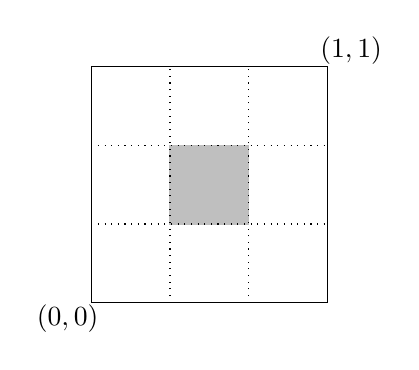
\begin{tikzpicture}[auto,scale = 1]
\draw (0,0) rectangle (3,3);
\draw [fill = gray!50,draw = gray!50] (1,1) rectangle (2,2);
\node (uf) at (3.5,1) {};
\node (0) at (-0.3,-0.2) {$(0,0)$};
\node (1) at (3.3,3.2) {$(1,1)$};
\draw [dotted] (1,0) to (1,3);
\draw [dotted] (2,0) to (2,3);
\draw [dotted] (0,1) to (3,1);
\draw [dotted] (0,2) to (3,2);
\end{tikzpicture}
\begin{tikzpicture}
\draw[color = white] (0,-1) rectangle (1.5,-1.1);
\end{tikzpicture}
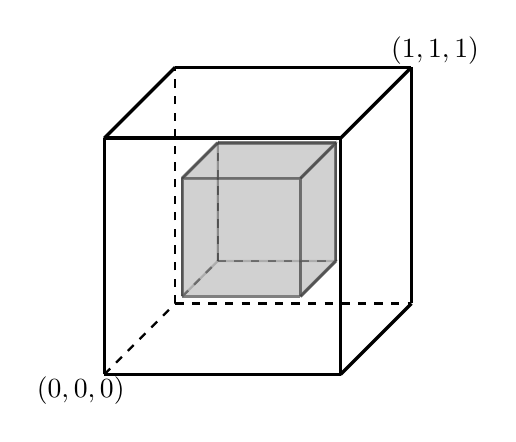
\begin{tikzpicture}[thick,scale=3]
	\node (0) at (-0.1,-0.07) {$(0,0,0)$};
	\node (1) at (1.4,1.37) {$(1,1,1)$};
    \coordinate (A1) at (0, 0);
    \coordinate (A2) at (0, 1);
    \coordinate (A3) at (1, 1);
    \coordinate (A4) at (1, 0);
    \coordinate (B1) at (0.3, 0.3);
    \coordinate (B2) at (0.3, 1.3);
    \coordinate (B3) at (1.3, 1.3);
    \coordinate (B4) at (1.3, 0.3);

    \draw[very thick] (A1) -- (A2);
    \draw[very thick] (A2) -- (A3);
    \draw[very thick] (A3) -- (A4);
    \draw[very thick] (A4) -- (A1);

    \draw[dashed] (A1) -- (B1);
    \draw[dashed] (B1) -- (B2);
    \draw[very thick] (A2) -- (B2);
    \draw[very thick] (B2) -- (B3);
    \draw[very thick] (A3) -- (B3);
    \draw[very thick] (A4) -- (B4);
    \draw[very thick] (B4) -- (B3);
    \draw[dashed] (B1) -- (B4);
    
    \coordinate (A13) at (0.33, 0.33);
    \coordinate (A23) at (0.33, 0.83);
    \coordinate (A33) at (0.83, 0.83);
    \coordinate (A43) at (0.83, 0.33);
    \coordinate (B13) at (0.48, 0.48);
    \coordinate (B23) at (0.48, 0.98);
    \coordinate (B33) at (0.98, 0.98);
    \coordinate (B43) at (0.98, 0.48);

    \draw[very thick,color = gray] (A13) -- (A23);
    \draw[very thick,color = gray] (A23) -- (A33);
    \draw[very thick,color = gray] (A33) -- (A43);
    \draw[very thick,color = gray] (A43) -- (A13);

    \draw[dashed,color = gray] (A13) -- (B13);
    \draw[dashed,color = gray] (B13) -- (B23);
    \draw[very thick,color = gray] (A23) -- (B23);
    \draw[very thick,color = gray] (B23) -- (B33);
    \draw[very thick,color = gray] (A33) -- (B33);
    \draw[very thick,color = gray] (A43) -- (B43);
    \draw[very thick,color = gray] (B43) -- (B33);
    \draw[dashed,color = gray] (B13) -- (B43);
    
    \draw[fill=gray,opacity = 0.2] (A13) -- (B13) -- (B43) -- (A43);
    \draw[fill=gray,opacity = 0.2] (A13) -- (A23) -- (A33) -- (A43);
    \draw[fill=gray,opacity = 0.2] (A13) -- (A23) -- (B23) -- (B13);
    \draw[fill=gray,opacity = 0.2] (B13) -- (B23) -- (B33) -- (B43);
    \draw[fill=gray,opacity = 0.2] (A33) -- (B33) -- (B43) -- (A43);
    \draw[fill=gray,opacity = 0.2] (A23) -- (B23) -- (B33) -- (A33);
    
\end{tikzpicture}
  		\end{center}
	\end{figure}

As shown in \cite{raussen10}, $\tracep{X_1}{(0,0)}{(1,1)}$ is a topological
space with two connected components, one is composed of the traces which have 
dihomotopy type of 
the path going up to the left of, then above the hole, the other component is
composed of the traces which have the dihomotopy type of the path going along the 
bottom of the hole then up on its right. Moreover, the two connected components of 
$\trace{X_1}{(0,0)}{(1,1)}$ are contractible ; it is thus homotopy equivalent
to two points. 

As shown again in \cite{raussen10}, $\tracep{X_2}{(0,0,0)}{(1,1,1)}$ is 
homotopy equivalent to the circle $S^1$: there is a unique dipath up
to dihomotopy, hence the trace space $\tracep{X_2}{(0,0,0)}{(1,1,1)}$ is connected, but
there is a finer structure of dihomotopies which accounts for the non
simple-connectness character of $\tracep{X_2}{(0,0,0)}{(1,1,1)}$. For example, a homotopy equivalence (to be defined soon) from $\tracep{X_2}{(0,0,0)}{(1,1,1)}$ to the boundary of a triangle is depicted here:
	\begin{figure}[H]
		\begin{center}
    			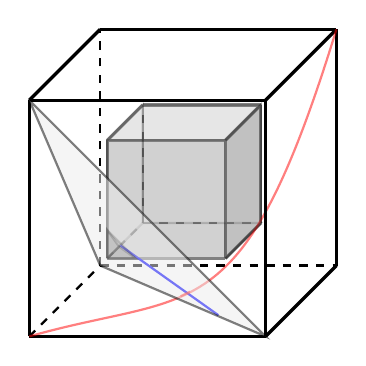
\begin{tikzpicture}[thick,scale=3]

    \coordinate (A1) at (0, 0);
    \coordinate (A2) at (0, 1);
    \coordinate (A3) at (1, 1);
    \coordinate (A4) at (1, 0);
    \coordinate (B1) at (0.3, 0.3);
    \coordinate (B2) at (0.3, 1.3);
    \coordinate (B3) at (1.3, 1.3);
    \coordinate (B4) at (1.3, 0.3);

    \draw[very thick] (A1) -- (A2);
    \draw[very thick] (A2) -- (A3);
    \draw[very thick] (A3) -- (A4);
    \draw[very thick] (A4) -- (A1);

    \draw[dashed] (A1) -- (B1);
    \draw[dashed] (B1) -- (B2);
    \draw[very thick] (A2) -- (B2);
    \draw[very thick] (B2) -- (B3);
    \draw[very thick] (A3) -- (B3);
    \draw[very thick] (A4) -- (B4);
    \draw[very thick] (B4) -- (B3);
    \draw[dashed] (B1) -- (B4);
    
    \coordinate (A13) at (0.33, 0.33);
    \coordinate (A23) at (0.33, 0.83);
    \coordinate (A33) at (0.83, 0.83);
    \coordinate (A43) at (0.83, 0.33);
    \coordinate (B13) at (0.48, 0.48);
    \coordinate (B23) at (0.48, 0.98);
    \coordinate (B33) at (0.98, 0.98);
    \coordinate (B43) at (0.98, 0.48);

    \draw[very thick,color = gray] (A13) -- (A23);
    \draw[very thick,color = gray] (A23) -- (A33);
    \draw[very thick,color = gray] (A33) -- (A43);
    \draw[very thick,color = gray] (A43) -- (A13);

    \draw[dashed,color = gray] (A13) -- (B13);
    \draw[dashed,color = gray] (B13) -- (B23);
    \draw[very thick,color = gray] (A23) -- (B23);
    \draw[very thick,color = gray] (B23) -- (B33);
    \draw[very thick,color = gray] (A33) -- (B33);
    \draw[very thick,color = gray] (A43) -- (B43);
    \draw[very thick,color = gray] (B43) -- (B33);
    \draw[dashed,color = gray] (B13) -- (B43);
    
    \draw[fill=gray,opacity = 0.2] (A13) -- (B13) -- (B43) -- (A43);
    
    \draw[blue] (0.385,0.385) -- (0.8,0.09);
    
    \draw[fill=gray,opacity = 0.2] (A13) -- (A23) -- (A33) -- (A43);
    \draw[fill=gray,opacity = 0.2] (A13) -- (A23) -- (B23) -- (B13);
    \draw[fill=gray,opacity = 0.2] (B13) -- (B23) -- (B33) -- (B43);
    \draw[fill=gray,opacity = 0.2] (A33) -- (B33) -- (B43) -- (A43);
    
     \draw[red, opacity = 0.5] (0,0) .. controls (0.7,0.2) and (0.9,0) .. (1.3,1.3);
    \draw[color = red,opacity = 0.5] (0.64,0.17) -- (0.68,0.19);
    \draw[fill = gray!15, opacity = 0.5] (A2) -- (A4) -- (B1) -- (A2);
    \draw[fill=gray,opacity = 0.2] (A43) -- (B43) -- (B33) -- (A33);
     \draw[fill=gray,opacity = 0.15] (A13) -- (0.38,0.38) -- (0.45,0.33) -- (A13);
     \draw[fill=gray,opacity = 0.15] (A13) -- (0.45,0.33) -- (0.33,0.45) -- (A13);
     \draw[fill=gray,opacity = 0.15] (A13) -- (0.38,0.38) -- (0.33,0.45) -- (A13);
     \draw[very thick] (A4) -- (A3);
\end{tikzpicture}
  		\end{center}
	\end{figure}






	